\documentclass[t, 10pt, mathserif]{beamer}

\usepackage[spanish]{babel}
\usepackage[utf8]{inputenc}
\usepackage{amscd}
\usepackage{amssymb}
\usepackage{amsthm}
\usepackage{latexsym}
\usepackage{setspace}
\usepackage{url}
\usepackage{xcolor}
\usepackage{bbm}

\mode<presentation>{
	\usecolortheme{}
	\useinnertheme{}
	\useoutertheme{}
}
\setbeamertemplate{sidebar right}{}
\setbeamertemplate{footline}{%
\hfill\usebeamertemplate***{navigation symbols}
\hspace{1cm}\insertframenumber{}/\inserttotalframenumber}

\beamertemplatenavigationsymbolsempty
\setbeamersize{text margin left = 1cm}
\setbeamertemplate{caption}[numbered]
\setbeamertemplate{frametitle}[default][left,leftskip=0.5cm]
\addtobeamertemplate{frametitle}{\vspace*{0.5cm}}{\vspace*{1cm}}

\setlength{\parskip}{\baselineskip}
\expandafter\def\expandafter\item\expandafter{\item \setlength{\parskip}{0.5\baselineskip}}
\expandafter\def\expandafter\definition\expandafter{\definition \setlength{\parskip}{0.5\baselineskip}}

\languagepath{spanish}
\deftranslation[to=spanish]{Corollary}{Corolario}
\deftranslation[to=spanish]{corollary}{corolario}
\deftranslation[to=spanish]{Definition}{Definición}
\deftranslation[to=spanish]{definition}{definición}
\deftranslation[to=spanish]{Lemma}{Lema}
\deftranslation[to=spanish]{lemma}{lema}
\deftranslation[to=spanish]{Problem}{Problema}
\deftranslation[to=spanish]{problem}{problema}
\deftranslation[to=spanish]{Theorem}{Teorema}
\deftranslation[to=spanish]{theorem}{teorema}
\newtheorem{belief}{Belief}
\newtheorem{conjecture}{Conjecture}
\newtheorem{observation}{Observation}
\newtheorem{question}{Question}

\newcommand {\base}[2]{\langle{#1};{#2}\rangle}
\newcommand{\abs}[1]{\left| #1 \right|}
\newcommand{\alocc}[2]{|\!|#1|\!|_{#2}}
\newcommand{\card}{\mbox{\raisebox{.13em}{{$\scriptstyle \#$}}}}
\newcommand{\ceil}[1]{\lceil #1 \rceil }
\newcommand{\cf}{\text{\em cf}}
\newcommand{\eps}{\varepsilon}
\newcommand{\expa}[1]{\{#1\}}
\newcommand{\floor}[1]{\lfloor #1 \rfloor } 
\newcommand{\N}{{\mathbb{N}}}
\newcommand{\NN}{\mathbb{N}}
\newcommand{\occ}[2]{|#1|_{#2}}
\newcommand{\Q}{{\mathbb{Q}}}
\newcommand{\R}{{\mathbb{R}}}
\newcommand{\RR}{\mathbb{R}}
\newcommand{\uno}{\mathbbm{1}}
\newcommand{\wh}[1]{\widehat{#1}}
\newcommand{\xbar}{{\overline{x}}}
\newcommand{\ybar}{{\overline{y}}}
\newcommand{\Z}{{\mathbb{Z}}}

\author{\large Emilio Almansi}

\begin{document}

\title{\normalsize Tesis de Licenciatura en Ciencias de la Computación \vspace*{1.5cm}}

\subtitle{\Large Secuencias completamente equidistribuidas basadas en secuencias de De Bruijn}

\date{
  {\footnotesize
    \hspace*{-6cm}
    \begin{tabular}{l}
      Directora: Verónica Becher \\
      Departamento de Computación\\
      Facultad de Ciencias Exactas y Naturales\\
      Universidad de Buenos Aires\\
      4 de septiembre, 2019
    \end{tabular}
  }
}

%%%%%%%%%%%%%%%%%%%%%%%%%%%%%%%%%%%%%%%%%%%%%%%%%%%%%%%%%%%%%%%%%%%

\begin{frame}
  \vspace{0.5cm}
  \maketitle
  \setcounter{framenumber}{0}
  \thispagestyle{empty}
\end{frame}

%%%%%%%%%%%%%%%%%%%%%%%%%%%%%%%%%%%%%%%%%%%%%%%%%%%%%%%%%%%%%%%%%%%

\begin{frame}
  \frametitle{Sobre secuencias aleatorias {$^{(1)}$}}

  ¿Qué tienen en común las siguientes áreas?
  \pause

  \begin{itemize}
    \item Criptografía, seguridad informática.\pause
    \item Predicción del clima, medicina nuclear, simulación de proteínas.\pause
    \item Aprendizaje automático, algoritmos probabilistas.\pause
    \item Juegos de azar, videojuegos, simulaciones físicas.
  \end{itemize}
  \pause

  {\color{orange} Generación de números aleatorios.}
  \pause

  Pero, ¿qué es una secuencia de números aleatorios?
\end{frame}

%%%%%%%%%%%%%%%%%%%%%%%%%%%%%%%%%%%%%%%%%%%%%%%%%%%%%%%%%%%%%%%%%%%

\begin{frame}
  \frametitle{Sobre secuencias aleatorias {$^{(2)}$}}

  \textbf{Intuición}: si tiro un dado muchas veces seguidas, el resultado de cada tirada tiene que ser \textit{impredecible} y todo número del 1 al 6 tiene que ser \textit{equiprobable}.
  \pause

  Respecto a la parte de \textit{impredecible}:
  \begin{quote}
    If ``random`` means that the sequence satisfies no predictable rules, the title of this paper is contradictory.
    \begin{flushright}
      \small{Construction of a Random Sequence \\}
      \small{Donald Knuth, 1965}
    \end{flushright}
  \end{quote}
  \pause

  En este trabajo, nos enfocamos en la parte de \textit{equiprobable}.
  % Es posible construir secuencias determinísticas que cumplen con esta propiedad.
\end{frame}

%%%%%%%%%%%%%%%%%%%%%%%%%%%%%%%%%%%%%%%%%%%%%%%%%%%%%%%%%%%%%%%%%%%

\begin{frame}
  \frametitle{Equidistribución {$^{(1)}$}}

  \begin{definition}
    Dado un entero $b$, una secuencia de \textit{números enteros} $X = x_1, x_2, \dots$ del conjunto $\{ 0, 1, \dots, b - 1 \}$ es \textbf{equidistribuida} si todo valor posible aparece con frecuencia asintótica igual a $\frac{1}{b}$:
    \pause

    \begin{equation*}
      \begin{aligned}
        Pr \left( x_i = j \right) = \frac{1}{b} \hspace*{1cm} \text{para todo } j \in \{ 0, \dots, b - 1 \} \text{,}
      \end{aligned}
    \end{equation*}
    \pause

    donde $Pr(x_i = j) = \lim_{N \to \infty} \frac{1}{N} \sum_{i = 1}^{N} \sigma(x_i = j)$.
  \end{definition}
  \pause

  Ahora, definimos una noción equivalente para secuencias de números reales.
\end{frame}

%%%%%%%%%%%%%%%%%%%%%%%%%%%%%%%%%%%%%%%%%%%%%%%%%%%%%%%%%%%%%%%%%%%

\begin{frame}
  \frametitle{Equidistribución {$^{(2)}$}}

  \begin{definition}
    Una secuencia de \textit{números reales} $X = x_1, x_2, \dots$ en el intervalo unitario $\left[0, 1\right)$ es \textbf{equidistribuida} si, dado cualquier conjunto $I \subseteq \left[0, 1\right)$, la frecuencia asintótica con la que la secuencia toma valores en $I$ es igual a su tamaño:
    \pause

    \begin{equation*}
      \begin{aligned}
        Pr \left( x_i \in I\, \right) = \left| I\, \right| \hspace*{1cm} \text{para todo } I \subseteq \left[0, 1\right) \text{,}
      \end{aligned}
    \end{equation*}
    \pause

    donde $Pr \left( x_i \in I\, \right) = \lim_{N \to \infty} \frac{1}{N} \sum_{i = 1}^{N} \sigma(x_i \in I\,)$.
  \end{definition}
  \pause

  Si $X$ es equidistribuida en $[0, 1)$, entonces para cualquier $b$ la secuencia $Y = \left( \lfloor b x_i \rfloor \right)_{i = 1}^{\infty}$ es equidistribuida en $\{ 0, 1, \dots, b - 1 \}$.
\end{frame}

% %%%%%%%%%%%%%%%%%%%%%%%%%%%%%%%%%%%%%%%%%%%%%%%%%%%%%%%%%%%%%%%%%%%

\begin{frame}
  \frametitle{Equidistribución {$^{(3)}$}}

  \vspace{-0.5cm}
  \begin{figure}
    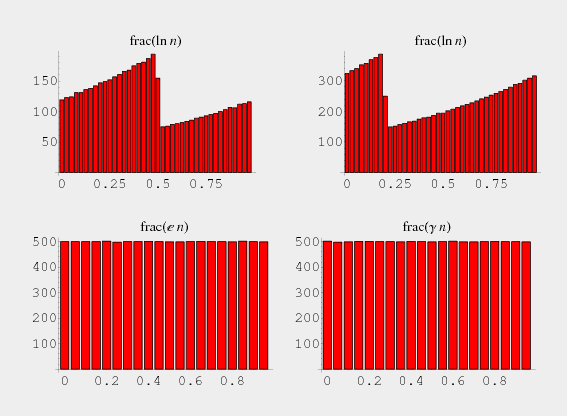
\includegraphics[width=0.7\textwidth]{resources/equidistribucion.png}
    \caption{Secuencias de partes fraccionarias.}
  \end{figure}
\end{frame}
 
%%%%%%%%%%%%%%%%%%%%%%%%%%%%%%%%%%%%%%%%%%%%%%%%%%%%%%%%%%%%%%%%%%%

\begin{frame}
  \frametitle{$k$-distribución {$^{(1)}$}}

  % Ahora extendemos la noción de equidistribución a otras dimensiones.
  % \pause

  \textbf{Intuición}: cualquier seguidilla de tiradas tiene que aparecer con igual frecuencia. Por ejemplo, (1, 1) aparece con la misma frecuencia que (2, 2) y que (6, 4).
  \pause

  Trabajamos con ``ventanas`` de tamaño $k$ de la secuencia. Si $X = x_1, x_2, \dots$ es una secuencia de \textit{números reales}, entonces:
  \pause

  \vspace{-0.3cm}
  \begin{equation*}
    \begin{aligned}
        w_1 & = (x_1, x_2, \dots, x_k      ), \\
        w_2 & = (x_2, x_3, \dots, x_{k + 1}), \\
        w_3 & = (x_3, x_4, \dots, x_{k + 2}), \\
            & \dots
    \end{aligned}
  \end{equation*}

  es la secuencia de ventanas de $X$, que llamamos $W_k(X)$.
\end{frame}

%%%%%%%%%%%%%%%%%%%%%%%%%%%%%%%%%%%%%%%%%%%%%%%%%%%%%%%%%%%%%%%%%%%

\begin{frame}
  \frametitle{$k$-distribución {$^{(2)}$}}

  \begin{definition}
    Una secuencia de \textit{números reales} $X = x_1, x_2, \dots$ en el intervalo unitario $\left[0, 1\right)$ es \textbf{$k$-distribuida} si, dado cualquier conjunto $I \subseteq \left[0, 1\right)^k$, la frecuencia asintótica con la que la secuencia de ventanas de $X$ toma valores en $I$ es igual a su tamaño:
    \pause

    \begin{equation*}
      \begin{aligned}
        Pr \left( w_i \in I\, \right) = \left| I\, \right| \hspace*{1cm} \text{para todo } I \subseteq \left[0, 1\right)^k \text{,}
      \end{aligned}
    \end{equation*}
    \pause

    \vspace{-0.5cm}
    \begin{equation*}
      \hspace{-2.5cm}
      \begin{aligned}
          \text{donde } W_k(X) =\; & \left( w_i \right)_{i = 1}^{\infty} \\
                               =\; & (x_1, x_2, \dots, x_k      ),\, (x_2, x_3, \dots, x_{k + 1}),\, \dots \, \text{.}
      \end{aligned}
    \end{equation*}
    \vspace{-0.3cm}
  \end{definition}
  \pause

  Si $X$ es $k$-distribuida para todo $k$, entonces $X$ es \textbf{completamente equidistribuida}.
\end{frame}

% %%%%%%%%%%%%%%%%%%%%%%%%%%%%%%%%%%%%%%%%%%%%%%%%%%%%%%%%%%%%%%%%%%%

\begin{frame}
  \frametitle{Equidistribución completa {$^{(1)}$}}

  ¿Por qué estudiar la propiedad de equidistribución?

  \begin{itemize}
    \item Requerimiento básico de pseudo-aleatoriedad. Propiedades de equipartición y autocorrelación con retraso. \pause
    \item Calidad de un generador de números aleatorios o PNRG. Pruebas de aleatoriedad.\pause % Mersenne Twister
    \item Integración de Montecarlo, criterio de la integral de Riemann. \pause
    \item Vínculo: teoría de números, computación, probabilidad y estadística.
  \end{itemize}
  \pause

  ¿Qué \textbf{no} es la equidistribución?
\end{frame}
 
% %%%%%%%%%%%%%%%%%%%%%%%%%%%%%%%%%%%%%%%%%%%%%%%%%%%%%%%%%%%%%%%%%%%

\begin{frame}
  \frametitle{Equidistribución completa {$^{(2)}$}}

  \vspace{-0.5cm}
  \begin{figure}
    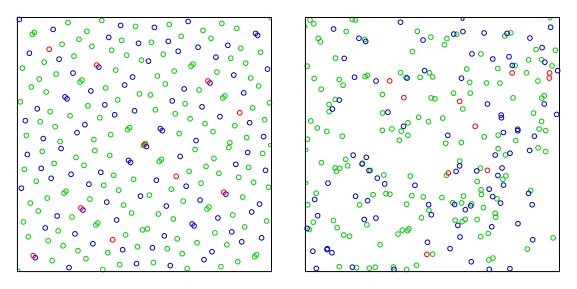
\includegraphics[width=0.8\textwidth]{resources/discrepancia.png}
    \caption{Izq.) Secuencia Sobol 2,3. Der.) Secuencia pseudo-aleat.}
  \end{figure}
\end{frame}
 
%%%%%%%%%%%%%%%%%%%%%%%%%%%%%%%%%%%%%%%%%%%%%%%%%%%%%%%%%%%%%%%%%%%

\begin{frame}{Secuencias de De Bruijn}
  \only<1->{
    Son secuencias muy estudiadas en combinatoria. Tienen la propiedad de ``contener`` a todas las posibles combinaciones de secuencias de un alfabeto y tamaño dados. Ejemplos:
  }

  \only<2->{Con $b = 2, k = 3$:}
  \only<2->{\vspace{-0.3cm}}
  \begin{center}
    \only<2>{$0, 0, 0, 1, 0, 1, 1, 1$}
    \only<3>{$\textbf{0, 0, 0}, 1, 0, 1, 1, 1$}
    \only<4>{$0, \textbf{0, 0, 1}, 0, 1, 1, 1$}
    \only<5>{$0, 0, \textbf{0, 1, 0}, 1, 1, 1$}
    \only<6>{$0, 0, 0, \textbf{1, 0, 1}, 1, 1$}
    \only<7>{$0, 0, 0, 1, \textbf{0, 1, 1}, 1$}
    \only<8>{$0, 0, 0, 1, 0, \textbf{1, 1, 1}$}
    \only<9>{$\textbf{0}, 0, 0, 1, 0, 1, \textbf{1, 1}$}
    \only<10>{$\textbf{0, 0}, 0, 1, 0, 1, 1, \textbf{1}$}
    \only<11->{$0, 0, 0, 1, 0, 1, 1, 1$}
    \only<11->{\vspace{-0.3cm}}
  \end{center}

  \only<11->{Con $b = 4, k = 2$:}
  \only<11->{\vspace{-0.3cm}}
  \begin{center}
    \only<12->{$0, 0, 1, 0, 2, 0, 3, 1, 1, 2, 1, 3, 2, 2, 3, 3$}
  \end{center}

  \only<13->{Notar que siempre tienen longitud $b^k$.}
  \only<14->{{\color{orange} ¿Qué relación tienen con las secuencias equidistribuidas?}}
\end{frame}

%%%%%%%%%%%%%%%%%%%%%%%%%%%%%%%%%%%%%%%%%%%%%%%%%%%%%%%%%%%%%%%%%%%

\begin{frame}
  \frametitle{Secuencia de Knuth {$^{(1)}$}}

  \vspace{-0.4cm}
  \begin{definition}
    Una \textbf{secuencia $A$ de órden $n$} es la secuencia que se obtiene al dividir cada elemento de una secuencia de De Bruijn de base $2^n$ y de órden $n$ por su base:
    \pause

    \vspace{-0.2cm}
    \begin{equation*}
      \begin{aligned}
        A^{(n)} & = \frac{f_1}{2^n}, \frac{f_2}{2^n}, \dots, \frac{f_{2^{n^2}}}{2^n}
      \end{aligned}
    \end{equation*}

    \vspace{-0.2cm}
    donde $F^{(2^n, n)} = f_1, \dots, f_{2^{n^2}}$ denota una secuencia de De Bruijn de base $2^n$ y de órden $n$.
    \pause

    Una \textbf{secuencia $B$ de órden $n$} es la secuencia que se obtiene de concatenar $n 2^{2 n}$ copias de una secuencia $A$ de órden $n$:
    \pause

    \vspace{-0.2cm}
    \begin{equation*}
      B^{(n)} = \left< \underbrace{A^{(n)} ; A^{(n)} ; \dots ; A^{(n)}}_{n 2^{2 n} \text{ veces}} \right> \text{.}
    \end{equation*}
  \end{definition}
\end{frame}


%%%%%%%%%%%%%%%%%%%%%%%%%%%%%%%%%%%%%%%%%%%%%%%%%%%%%%%%%%%%%%%%%%%

\begin{frame}
  \frametitle{Secuencia de Knuth {$^{(2)}$}}

  Ejemplo para $n = 2$:
  \pause

  \begin{equation*}
    \begin{aligned}
      F^{(4, 2)} & = 0, 0, 1, 0, 2, 0, 3, 1, 1, 2, 1, 3, 2, 2, 3, 3 \\[0.4cm] \pause
      A^{(2)}    & = \frac{0}{4}, \frac{0}{4}, \frac{1}{4}, \frac{0}{4}, \frac{2}{4}, \frac{0}{4}, \frac{3}{4}, \frac{1}{4}, \frac{1}{4}, \frac{2}{4}, \frac{1}{4}, \frac{3}{4}, \frac{2}{4}, \frac{2}{4}, \frac{3}{4}, \frac{3}{4} \\[0.4cm] \pause
      B^{(2)}   & = \left< \underbrace{A^{(2)} ; \dots ; A^{(2)}}_{2 \times 2^{2 \times 2} = 32 \text{ veces}} \right> \\[0.1cm] \pause
                & = \underbrace{\frac{0}{4}, \frac{0}{4}, \dots, \frac{3}{4}, \frac{3}{4}}_{A^{(2)}}, \dots, \underbrace{\frac{0}{4}, \frac{0}{4}, \dots, \frac{3}{4}, \frac{3}{4}}_{A^{(2)}} \text{.}
    \end{aligned}
  \end{equation*}
\end{frame}

%%%%%%%%%%%%%%%%%%%%%%%%%%%%%%%%%%%%%%%%%%%%%%%%%%%%%%%%%%%%%%%%%%%

\begin{frame}
  \frametitle{Secuencia de Knuth {$^{(3)}$}}

  Ahora sí, ya estamos en condiciones de definir la secuencia de Knuth.
  \pause

  \medskip
  \begin{definition}
    La secuencia de Knuth, que denominamos $K$, se define como la concatenación de todas las posibles secuencias $B$ en órden creciente:
    \pause

    \begin{equation*}
      K = \left< B^{(1)} ; B^{(2)} ;  B^{(3)} ; \dots \right> \text{.}
    \end{equation*}
  \end{definition}
  \pause

  \medskip
  \begin{theorem}[{{\scriptsize  Knuth, 1965}}]
    \medskip
    La secuencia $K$ es completamente equidistribuida.
  \end{theorem}
\end{frame}

% %%%%%%%%%%%%%%%%%%%%%%%%%%%%%%%%%%%%%%%%%%%%%%%%%%%%%%%%%%%%%%%%%%%

\begin{frame}{Secuencia de Knuth {$^{(4)}$}}
  \vspace{-0.5cm}
  \only<1>{
    \begin{figure}
      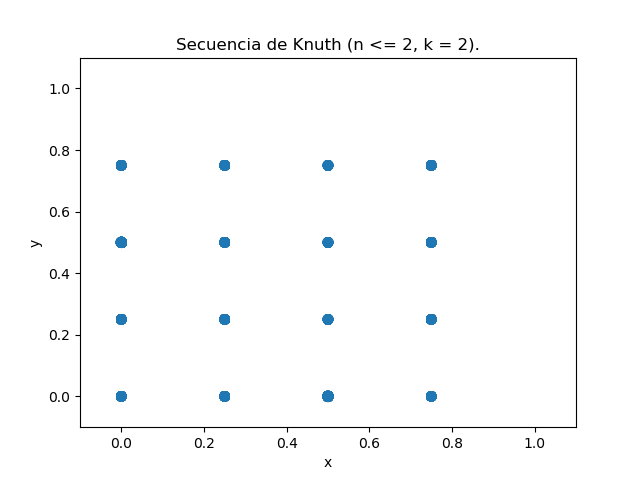
\includegraphics[width=0.7\textwidth]{resources/secuencia-knuth-1.png}
      \caption{Secuencia de Knuth en dos dimensiones.}
    \end{figure}
  }
  \only<2>{
    \begin{figure}
      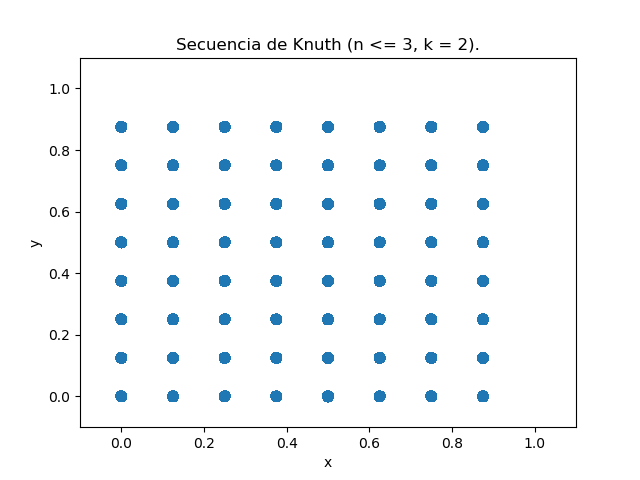
\includegraphics[width=0.7\textwidth]{resources/secuencia-knuth-2.png}
      \caption{Secuencia de Knuth en dos dimensiones.}
    \end{figure}
  }
\end{frame}
 
%%%%%%%%%%%%%%%%%%%%%%%%%%%%%%%%%%%%%%%%%%%%%%%%%%%%%%%%%%%%%%%%%%%

\begin{frame}
  \frametitle{Idea de la demostración}

  Mauris euismod neque a lorem rutrum, id molestie eros consequat.
  \pause
  
  In facilisis magna eu libero commodo, id tincidunt {\color{magenta} $\ell$} purus pellentesque.
  \pause

  \medskip
  \begin{definition}
    Fusce sit amet lacus viverra, viverra massa sit amet, placerat neque. Integer ipsum sapien, efficitur quis dui vitae, facilisis tempus dolor.
    \pause

    Duis ornare volutpat libero, at sodales dolor porttitor at.
    \pause
  \end{definition}

  In rutrum dapibus justo, at mattis lacus ultrices sed. Suspendisse suscipit luctus fermentum.
\end{frame}

%%%%%%%%%%%%%%%%%%%%%%%%%%%%%%%%%%%%%%%%%%%%%%%%%%%%%%%%%%%%%%%%%%%

\begin{frame}
  \frametitle{Alfabetos linealmente crecientes}

  \vspace{-0.4cm}
  \begin{definition}
    Una \textbf{secuencia $C$ de órden $n$} es la secuencia que se obtiene al dividir cada elemento de una secuencia de De Bruijn de base $n$ y de órden $n$ por su base:
    \pause

    \vspace{-0.2cm}
    \begin{equation*}
      \begin{aligned}
        C^{(n)} & = \frac{f_1}{n}, \frac{f_2}{n}, \dots, \frac{f_{n^n}}{n}
      \end{aligned}
    \end{equation*}

    \vspace{-0.2cm}
    donde $F^{(n, n)} = f_1, \dots, f_{n^n}$ denota una secuencia de De Bruijn de base $n$ y de órden $n$.
    \pause

    Una \textbf{secuencia $D$ de órden $n$} es la secuencia que se obtiene de concatenar $t(n)$ copias de una secuencia $C$ de órden $n$:
    \pause

    \vspace{-0.2cm}
    \begin{equation*}
      D^{(n)} = \left< \underbrace{C^{(n)} ; C^{(n)} ; \dots ; C^{(n)}}_{t(n) \text{ veces}} \right> \text{.}
    \end{equation*}
  \end{definition}
\end{frame}

%%%%%%%%%%%%%%%%%%%%%%%%%%%%%%%%%%%%%%%%%%%%%%%%%%%%%%%%%%%%%%%%%%%

\begin{frame}
  \frametitle{Alfabetos linealmente crecientes}

  \vspace{-0.4cm}
  \begin{definition}
    Una \textbf{secuencia $C$ de órden $n$} es la secuencia que se obtiene al dividir cada elemento de una secuencia de De Bruijn de {\color{orange} base $n$} y de órden $n$ por su base:

    \vspace{-0.2cm}
    \begin{equation*}
      \begin{aligned}
        C^{(n)} & = \frac{f_1}{{\color{orange} n}}, \frac{f_2}{{\color{orange} n}}, \dots, \frac{f_{{\color{orange} n^n}}}{{\color{orange} n}}
      \end{aligned}
    \end{equation*}

    \vspace{-0.2cm}
    donde $F^{({\color{orange} n}, n)} = f_1, \dots, f_{{\color{orange} n^n}}$ denota una secuencia de De Bruijn de base $n$ y de órden $n$.

    Una \textbf{secuencia $D$ de órden $n$} es la secuencia que se obtiene de concatenar {\color{orange} $t(n)$ copias} de una secuencia $C$ de órden $n$:

    \vspace{-0.2cm}
    \begin{equation*}
      D^{(n)} = \left< \underbrace{C^{(n)} ; C^{(n)} ; \dots ; C^{(n)}}_{{\color{orange} t(n)} \text{ veces}} \right> \text{.}
    \end{equation*}
  \end{definition}
\end{frame}

%%%%%%%%%%%%%%%%%%%%%%%%%%%%%%%%%%%%%%%%%%%%%%%%%%%%%%%%%%%%%%%%%%%

\begin{frame}
  \frametitle{Secuencia $L$ {$^{(1)}$}}

  \begin{definition}
    La secuencia $L$ se define como la concatenación de todas las posibles secuencias $D$ en órden creciente:
    \pause

    \begin{equation*}
      L = \left< D^{(1)} ; D^{(2)} ;  D^{(3)} ; \dots \right> \text{.}
    \end{equation*}
  \end{definition}
  \pause

  {\color{orange} Ahora, enunciamos el aporte principal de esta tesis.}
  \pause

  \medskip
  \begin{block}{Teorema 1}
    \medskip
    \textit{Si $t : \mathbb{N} \mapsto \mathbb{N}$ es una función no decreciente y $\lim_{n \to \infty} n / t(n) = 0$, entonces la secuencia $L$ es completamente equidistribuida.}
  \end{block}
\end{frame}

% %%%%%%%%%%%%%%%%%%%%%%%%%%%%%%%%%%%%%%%%%%%%%%%%%%%%%%%%%%%%%%%%%%%

\begin{frame}{Secuencia $L$ {$^{(2)}$}}
  \vspace{-0.5cm}
  \only<1>{
    \begin{figure}
      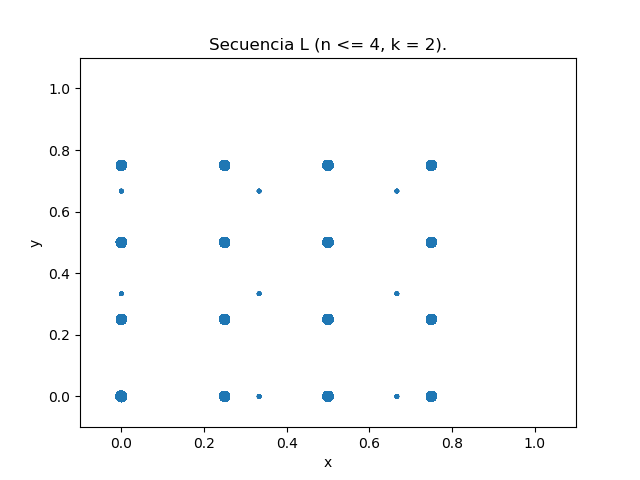
\includegraphics[width=0.7\textwidth]{resources/secuencia-l-1.png}
      \caption{Secuencia $L$ en dos dimensiones.}
    \end{figure}
  }
  \only<2>{
    \begin{figure}
      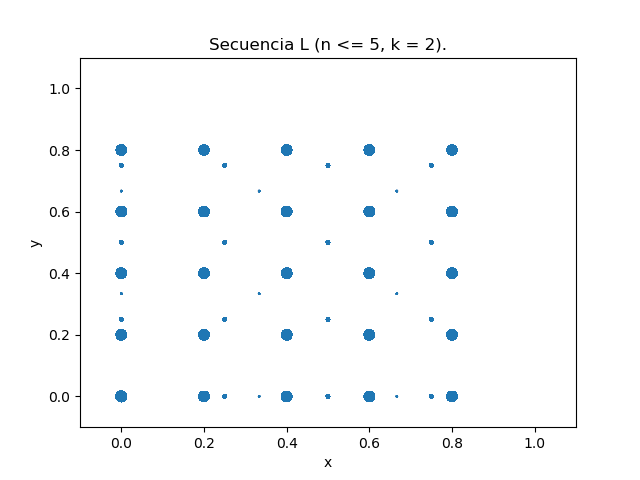
\includegraphics[width=0.7\textwidth]{resources/secuencia-l-2.png}
      \caption{Secuencia $L$ en dos dimensiones.}
    \end{figure}
  }
\end{frame}
 
%%%%%%%%%%%%%%%%%%%%%%%%%%%%%%%%%%%%%%%%%%%%%%%%%%%%%%%%%%%%%%%%%%%

\begin{frame}
  \frametitle{Idea de la demostración}

  Mauris euismod neque a lorem rutrum, id molestie eros consequat.
  \pause
  
  In facilisis magna eu libero commodo, id tincidunt {\color{magenta} $\ell$} purus pellentesque.
  \pause

  \medskip
  \begin{definition}
    Fusce sit amet lacus viverra, viverra massa sit amet, placerat neque. Integer ipsum sapien, efficitur quis dui vitae, facilisis tempus dolor.
    \pause

    Duis ornare volutpat libero, at sodales dolor porttitor at.
    \pause
  \end{definition}

  In rutrum dapibus justo, at mattis lacus ultrices sed. Suspendisse suscipit luctus fermentum.
\end{frame}

%%%%%%%%%%%%%%%%%%%%%%%%%%%%%%%%%%%%%%%%%%%%%%%%%%%%%%%%%%%%%%%%%%%

\begin{frame}
  \frametitle{Prueba alternativa {$^{(1)}$}}

  Presentamos una prueba alternativa más sencilla, basada en el criterio de Weyl y en una proposición de la teoría de congruencias lineales.
  \pause

  \medskip
  \begin{block}{Criterio de Weyl}
    \medskip
    Una secuencia $X = x_1, x_2, \dots$ de números reales en $[0, 1)$ es $k$-distribuida si, y solo si, para cualquier vector de enteros no nulo $\bar{\ell} = (l_1, \dots, l_k)$:
    \pause

    \begin{equation*}
      \lim_{N \to \infty} \frac{1}{N} \sum_{n = 1}^{N} e^{2 \pi i \bar{\ell} \cdot \bar{w}_n} = 0 \text{,}
    \end{equation*}

    donde $W_k(X) = \bar{w}_1, \bar{w}_2, \dots$ es la secuencia de ventanas de órden $k$ de $X$.
  \end{block}
  \pause

  Podemos reducir el problema a una cota sobre una suma exponencial.
\end{frame}

%%%%%%%%%%%%%%%%%%%%%%%%%%%%%%%%%%%%%%%%%%%%%%%%%%%%%%%%%%%%%%%%%%%

\begin{frame}
  \frametitle{Prueba alternativa {$^{(2)}$}}

  Mauris euismod neque a lorem rutrum, id molestie eros consequat.
  \pause
  
  In facilisis magna eu libero commodo, id tincidunt {\color{magenta} $\ell$} purus pellentesque.
  \pause

  \medskip
  \begin{definition}
    Fusce sit amet lacus viverra, viverra massa sit amet, placerat neque. Integer ipsum sapien, efficitur quis dui vitae, facilisis tempus dolor.
    \pause

    Duis ornare volutpat libero, at sodales dolor porttitor at.
    \pause
  \end{definition}

  In rutrum dapibus justo, at mattis lacus ultrices sed. Suspendisse suscipit luctus fermentum.
\end{frame}

%%%%%%%%%%%%%%%%%%%%%%%%%%%%%%%%%%%%%%%%%%%%%%%%%%%%%%%%%%%%%%%%%%%

\begin{frame}
  \frametitle{Problemas abiertos}

  Quedan varias líneas claras de investigación futura:
  \pause

  \begin{itemize}
    \item ¿Qué pasa cuando no se cumple que $\lim_{n \to \infty} n / t(n) = 0$? ¿La secuencia $L$ sigue siendo completamente equidistribuida?
    \pause
    
    \item Para responder eso, es necesario entender mejor la discrepancia de la familia de secuencias de De Bruijn que se use para formar la secuencia $L$.
    \pause

    \item Relacionado: ¿cumple la secuencia $L$ la propiedad de correlación de pares de Poisson?
  \end{itemize}
\end{frame}

\newcounter{finalframe}
\setcounter{finalframe}{\value{framenumber}}

% \addtocounter{framenumber}{-1}

% \begin{frame}
% \scriptsize

% \begin{thebibliography}{1}

% \setlength{\parskip}{-0.5mm}

% \bibitem{agafonov1968normal}
% V.~N. Agafonov.
% \newblock Normal sequences and finite automata.
% \newblock {\em Soviet Mathematics Doklady}, 9:324--325, 1968.

% \bibitem{BecherCarton2017}
% Ver\'onica Becher and Olivier Carton.
% \newblock Normal numbers and computer science.
% \newblock In Val\'erie Berth\'e and Michel Rig\'o, editors, {\em Sequences,
%   Groups, and Number Theory}, Trends in Mathematics Series.
%   Birkhauser/Springer, 2017.

% \bibitem{borel1909probabilites}
% {\'E}mile Borel.
% \newblock Les probabilit{\'e}s d{\'e}nombrables et leurs applications
%   arithm{\'e}tiques.
% \newblock {\em Rendiconti del Circolo Matematico di Palermo}, 27(1):247--271,
%   1909.

% \bibitem{bugeaud2012distribution}
% Yann Bugeaud.
% \newblock {\em Distribution modulo one and Diophantine approximation}, volume
%   193.
% \newblock Cambridge University Press, 2012.

% \bibitem{Champernowne:1933}
% David Champernowne.
% \newblock The {C}onstruction of {D}ecimals {N}ormal in the {S}cale of {T}en.
% \newblock {\em The Journal of the London Mathematical Society},
%   s1-8(4):254--260, 1933.

% \bibitem{rogers1987theory}
% Jr. Hartley~Rogers.
% \newblock {\em Theory of recursive functions and effective computability}.
% \newblock MIT Press, Cambridge, MA, second edition, 1987.

% \bibitem{kamae1975normal}
% Teturo Kamae and Benjamin Weiss.
% \newblock Normal numbers and selection rules.
% \newblock {\em Israel Journal of Mathematics}, 21(2):101--110, 1975.

% \bibitem{Piatetski-Shapiro:1951}
% I.~I. Piatetski-Shapiro.
% \newblock On the law of distribution of the fractional parts of the exponential
%   function.
% \newblock {\em Izv. Akad. Nauk SSSR Ser. Mat.}, 15(1):47--52, 1951.

% \bibitem{vandehey2016uncanny}
% Joseph Vandehey.
% \newblock Uncanny subsequence selections that generate normal numbers.
% \newblock {\em ar{X}iv:1607.03531}, 2016.
% \end{thebibliography}

% \end{frame}

\end{document}
